\section{Análise de Ruído das operações}

\subsection{Operações RGSW}
Nesta seção estão as análises do crescimento de ruído das operações entre criptogramas RGSW.
\subsubsection{Soma Homomórfica $C_1 \boxplus  C_2$}
O ruído dessa operação pode ser calculado por:
$$
Err(C_1 \boxplus  C_2) = sk^T(C_1 + C_2) - (\mu_1 + \mu_2)sk^TG
$$
Organizando,
$$
Err(C_1 \boxplus  C_2) = sk^T(C_1) - (\mu_1)sk^TG + sk^T(C_2) - (\mu_2)sk^TG = e_1^T + e_2^T 
$$

\subsubsection{Multiplicação Homomórfica $C_1 \boxdot C_2$}
O ruído desta operação pode ser calculado por
$$
Err(C_1 \boxdot C_2) = sk^\top(C_1G ^{-1}(C_2)) - (\mu_1\mu_2)sk^\top \mathbf{G}
$$
Expandindo a expressão encontra-se:
$$
Err(C_1 \boxdot C_2) = (1,-s) \begin{pmatrix} s \mathbf{a}_1^\top + \mathbf{e}_1^\top \\ \mathbf{a}_ 1^\top \end{pmatrix}G ^{-1}(C_2) + \mu_1(1,-s)\begin{pmatrix} s \mathbf{a}_2^\top + \mathbf{e}_2^\top \\ \mathbf{a}_ 2^\top \end{pmatrix}
$$
Simplificando, finalmente:
$$
Err(C_1 \boxdot C_2) = \mathbf{e}_1^\top G ^{-1}(C_2) + \mu_1 \mathbf{e}_2^\top
$$

\subsection{Ext-Prod}
O produto externo entre RGSW e RLWE pode ser calculado por

$$C_1 \boxtimes c_2 = \begin{pmatrix} s \mathbf{a}_1^\top + \mathbf{e}_1^\top \\ \mathbf{a}_ 1^\top \end{pmatrix}g^{-1}(c_2) + \mu_1\mathbf{G}g^{-1}(c_2)$$ 
$$=\begin{pmatrix} s \mathbf{a}_1^\top g^{-1}(c_2) + \mathbf{e}_1^\top g^{-1}(c_2) \\ \mathbf{a}_ 1^\top g^{-1}(c_2) \end{pmatrix} + \begin{pmatrix} s a_2 \mu_1 + \mu_1 \mu_2 \frac{Q}{B} + \mu_1 e_2 \\ a_2 \mu_1 \end{pmatrix} $$
$$=\begin{pmatrix} s ( \mathbf{a}_1^\top g^{-1}(c_2) + a_2\mu_1) + \mu_1\mu_2\frac{Q}{B} +  \mathbf{e}_1^\top g^{-1}(c_2) +\mu_1 e_2 \\ \mathbf{a}_ 1^\top g^{-1}(c_2) + a_2 \mu_1 \end{pmatrix}$$
Finalmente, o ruído é calculado por:
$$
Err(C_1 \boxtimes c_2) = \mathbf{e}_1^\top g^{-1}(c_2) +\mu_1 e_2  
$$
Dessa forma, a sua norma infinita deve ser
$$
||Err(C_1 \boxtimes c_2)||_\infty < 2\ell N||e_1||_\infty + \mu_1 ||e_2||_\infty 
$$

\subsection{Subgaussiana}
Para a análise de ruído 'justa' é preciso utilizar que parte das variáveis aleatórias trabalhadas são limitadas por distribuições 
subgaussianas. A intuição é de que podemos encontrar um limite superior probabilístico utilizando a desigualdade de Markov se soubermos
a distribuição que rege a variável aleatória. 

\begin{definition}
    Para \( s > 0 \), define-se a função Gaussiana \( \rho_s : H \to (0,1] \) por
\[
\rho_s(\mathbf{x}) = \exp\left(-\pi \|\mathbf{x}\|_2^2 / s^2\right).
\]
A distribuição Gaussiana contínua \( D_s \) é obtida pela normalização de \( \rho_s \), com densidade \( s^{-n} \cdot \rho_s(\mathbf{x}) \).

Define-se também que uma variável aleatória \( X \in \mathbb{R} \) é \( \delta \)-subgaussiana com parâmetro \( s > 0 \) se, para todo \( t \in \mathbb{R} \),
\[
\mathbb{E}[\exp(2\pi t X)] \leq \exp(\delta + \pi s^2 t^2).
\]

\end{definition}

Agora tome as seguintes propriedades presentes em \cite{lyubashevsky2013} e \cite{lw23I}.

\begin{lemma}[Lema 3.2 \cite{lw23I}]
    \textit{Para quaisquer cifras RGSW} $\mathbf{C}_1, \mathbf{C}_2$ \textit{que cifram} $\mu_1, \mu_2$ \textit{com termos de erro} $\mathbf{e}_1, \mathbf{e}_2$ \textit{respectivamente, temos o seguinte:}

    \[
    \text{Err}(\mathbf{C}_1 \boxplus \mathbf{C}_2) = \mathbf{e}_1^\top + \mathbf{e}_2^\top.
    \]

    \[
    \text{Err}(\mathbf{C}_1 \boxtimes \mathbf{C}_2) = \mathbf{e}_1^\top \cdot \mathbf{G}^{-1}(\mathbf{C}_2) + \mu_1 \cdot \mathbf{e}_2^\top.
    \]

    \textit{Além disso, suponha que} $\mathbf{G}^{-1}$ \textit{é amostrado com respeito a alguma base} $\mathbb{Z}$ \textit{de} $\mathcal{R}$, \textit{isto é,} $\mathbf{B} = \{ \mathbf{b}_1, \dots, \mathbf{b}_n \}$, \textit{tal que} $\max_{i \in [n]} \{ \| \sigma(\mathbf{b}_i) \|_\infty \} \leq 1$ \textit{como no Lema 2.3. Então os seguintes fatos valem:}

    \begin{itemize}
    \item Denote $\mathbf{e}_1^\top \cdot \mathbf{G}^{-1}(\mathbf{C}_2)$ como $\mathbf{e}^\top = (e_1, \dots, e_{2\ell})$. Então cada entrada de $\mathbf{e}$ é uma variável aleatória independente.

    \item $\|\sigma(\mathbf{e})\|_\infty$ é limitada superiormente por uma variável sub-Gaussiana com parâmetro $O(r)$, para algum $r > 0$ tal que $r \leq \sqrt{N \cdot \log Q} \cdot \|\sigma(\mathbf{e}_1)\|_\infty$.
    \end{itemize}
\end{lemma}


\begin{lemma}
    Seja uma variável aleatória $X$ de distribuição gaussiana de parâmetros $(\mu = 0, \sigma)$, esta variável é limitada superiormente
    por um subgaussiana de parâmetro mínimo $\sqrt{2\pi}\sigma$
\end{lemma}
\begin{proof}
    Basta computar $\mathbb{E}[2\pi tX]$
    $$
    \mathbb{E}[2\pi tX] = \int_{-\infty}^{\infty} Ae^{-\frac{1}{2\sigma^2}X^2} e^{2\pi tX}  dX
    $$
    $$
    \int_{-\infty}^{\infty} Ae^{-\frac{1}{2\sigma^2}X^2} e^{2\pi tX}dX  = \int_{-\infty}^{\infty} Ae^{-\frac{1}{2\sigma^2}X^2} e^{2\pi tX} e^{2\pi \sigma^2 t^2} e^{-2\pi \sigma^2 t^2}dX
    $$
    $$
    \mathbb{E}[2\pi tX] = \int_{-\infty}^{\infty} Ae^{-\frac{1}{2\sigma^2}(X - 2\pi \sigma^2 t)^2}  e^{2\pi^2 \sigma^2 t^2} dX
    $$
    Como a segunda exponencial não depende de $X$, 
    $$
    \mathbb{E}[2\pi tX] = e^{2\pi^2 \sigma^2 t^2} \int_{-\infty}^{\infty} Ae^{-\frac{1}{2\sigma^2}(X - 2\pi \sigma^2 t)^2} dX
    $$
    Note porém que a integral agora toma a forma, $\int_{-\infty}^{\infty} Ae^{-\frac{1}{2\sigma^2}(X - \mu)^2} dX$, ou seja,
    é apenas a função de probabilidade de uma gaussiana deslocada da origem integrada em sua completude, logo resulta em $1$.
    Perceba que o processo anterior também funciona para uma gaussiana discreta, afinal se baseia apenas no processo de se aproveitar
    da normalização e do comportamento exponencial da gaussiana. Finalmente, para que seja uma distribuição subgaussiana de parâmetro $s$
    $$
    \mathbb{E}[2\pi tX] = e^{2\pi^2 \sigma^2 t^2} \le e^\delta e^{\pi s^2 t^2}
    $$
    Como o intuito é que a desigualdade seja válida para qualquer $t$, basta que $ 2\pi^2 \sigma^2 t^2 \le \pi s^2 t^2 \Rightarrow 2\pi \sigma^2 \le s^2 \Rightarrow s \ge \sigma \sqrt{2\pi}$
    Chegando assim no resultado desejado. 


\end{proof}

Agora, podemos passar para uma análise dos ruídos acumulados pelas operações.

\subsection{Key Switch}
O algoritmo de key-switch, como presente no nome, tem como função a troca de um criptograma cifrado
em uma chave antiga $s'$, para uma chave nova $s$, o que aumenta o ruído gerado na cifra, vamos verificar o quanto.
Para que o algortimo seja realizado corretamente, é necessário 
que seja passado como parâmetro a \textit{lower half} de um criptograma $RGSW_s(s')$, ou seja, é necessário assumir 
que o RGSW tem segurança circular.

Seja então $d \in \text{RLWE}_{s'}(\mu)$ e $d = (a, b)$, e queremos então um criptograma de $\mu$ cifrado em $\text{RLWE}_{s}$.
Considere então $K$ a \textit{lower half} de um criptograma $RGSW_s(s')$. O objetivo então é encontrar o ruído,
$$
[0,b] - K \times g^{-1}(a)
$$
Como $K$ é a parte inferior de $RGSW_s(s')$ considere $K = (A, As + gs' + \mathbf{e}_{KS}) \in \mathcal{R}_Q^{2 \times \ell}$. Aplicando na expressão anterior:  

$$
(g^{-1}(a) \times A),  (g^{-1}(a) \times A) s + s' g g^{-1}(a) + \mathbf{e}_{KS} g^{-1}(a)
$$
Utilizando a definição de $g$, $g g^{-1}(a) = a$, e subtraindo pelo vetor $[0, b]$, sabendo que $b = s'a + \mu \left\lfloor \frac{Q}{B} \right\rceil + E$:

$$
-(g^{-1}(a) \times A), -(g^{-1}(a) \times A) s + \mu \frac{Q}{B} + E - \mathbf{e}_{KS} g^{-1}(a)
$$
Note que o vetor obtido é um criptograma valido $\in \text{RLWE}_{s}(\mu)$ com ruído 
$$E - \mathbf{e}_{KS} g^{-1}(a)$$
onde $E$ é o ruído inicial do criptograma e $\mathbf{e}_{KS}$ é o vetor de ruído utilizado para cifrar $s$. Então, a norma infinita 
do ruído key-switch é: 

$$
||Err(KS(d))||_\infty < ||Err(d)||_\infty + N\ell ||\mathbf{e}_{KS}||_\infty
$$
No teorema 4.6 do \cite{lw23I}, assume-se que $Err(d)$ e $\mathbf{e}_{KS} g^{-1}(a)$ são subgaussianas com um mesmo parametro $B$, o que faz sentido 
visto que a magnitude do ruído do key-switch deve ser muito menor do que a da mensagem $d$.

\subsection{Eval-Trace}

Para a análise de ruído do algoritmo 4.1 de \cite{lw23I}. Para facilitar a análise, considere o mesmo
algoritmo simplificado, para o efeito da acumulação do ruído ser mais visível, a variável $d$ terá um 
índice que representa seu degrau na torre de extensão. 

\begin{algorithm}[H]
\caption{(RLWE)-Eval-Tr\(_{K/K_{13}}\) com a estrutura de torre}
\SetKwInOut{Input}{Entrada}
\SetKwInOut{Output}{Saída}

\Input{
\begin{itemize}
  \item \(c = (b, a) \in (\mathcal{R}_1 \otimes \mathcal{R}_2 \otimes \mathcal{R}_3)^2\) que encripta uma mensagem \(\mu \in \mathcal{R}_1 \otimes \mathcal{R}_2 \otimes \mathcal{R}_3\) sob um segredo \(s \in \mathcal{R}\).
  \item \(\{\text{evk}^{(\sigma)}\}_{\sigma \in \bigcup_{i=1}^{t-1} \text{Gal}(E_i/E_{i+1})}\), e \(\text{evk} \in \text{RGSW}_s(P^{-1} \cdot s) \in \mathcal{R}^2\).
\end{itemize}
}
\Output{
\(c_{out} \in \text{RLWE}_s(\text{Tr}_{K/K_{13}}(\mu))\).
}

Inicialize \(c = (b, a)\), defina \(\bar{a} = P \cdot a\) \\
Calcule \(d_0 = \text{evk} \boxtimes (0, \bar{a})\) \\
\For{\(i = 1\) até \(t - 1\)}{
  Calcule \(d_{i+1} = \sum_{\sigma \in \text{Gal}(E_i/E_{i+1})} \text{KS}( \sigma(d_i), \text{evk}^{(\sigma^{-1})})\)\\
}
Retorne \((\text{Tr}_{K/K_{13}}(b), 0) - d_n\) 

\end{algorithm}
Assuma sem perda de generalidade que o traço realizado é $K \rightarrow K_{13}$.
Começaremos analisando a recurssão do loop na linha 4:
$$
d_{i+1} = \sum_{\sigma \in \text{Gal}(E_i/E_{i+1})} \text{KS}( \sigma(d_i), \text{evk}^{(\sigma^{-1})})
$$
Então, utilizando a expressão do erro do key-switch:
$$
Err(d_{i+1}) = \sum_{\sigma \in \text{Gal}(E_i/E_{i+1})} Err(\sigma(d_i)) - e_{KS}^{\sigma} g^{-1}(d_i[0])
$$
Perceba que $Err(\sigma(d_i)) = \sigma(Err(d_i))$ e que o segundo termo no somatório tem sua norma limitada por um valor pequeno,
em uma análise inicial $N\ell ||e_{KS}^{\sigma}||$, utilizando o lema 3.2 é uma variável subgaussiana com parâmetro limitado por 
$\sqrt{N\ell} ||e_{KS}^{\sigma}||$. Visto que sua norma independe do seu estágio na torre, troque-o por $e'$ onde $||e'|| \le  N\ell ||e_{KS}^{\sigma}||$.
$$
Err(d_{i+1}) < p_2 e'+ \sum_{\sigma \in \text{Gal}(E_i/E_{i+1})} \sigma(Err(d_i))
$$
Observe que o termo $\sum_{\sigma \in \text{Gal}(E_i/E_{i+1})} \sigma(Err(d_i)) = Tr_{E_i / E_{i+1}}(Err(d_i))$ 
$$
Err(d_{i+1}) < p_2 e' + Tr_{E_i/E_{i+1}}(Err(d_i))
$$
A partir dessa recorrência, é possível chegar na relação:
$$
Err(d_{n}) < Tr_{K/K_{13}}(Err(d_0)) + e' (p_2-1) \sum_{i=0}^{n_2-1} p_2^i < Tr_{K / K_{13}}(Err(d_0)) + \rho' e'
$$
Logo,
$$
Err(d_{n}) < Tr_{K / K_{13}}(Err(d_0)) + \rho' e'
$$
Sabendo que $d_0 = evk \boxtimes [0, \bar{a}]$, $Err(d_0) = Err(evk) g^{-1}([0, \bar{a}])$.
Tome $f$ como o criptograma resultante, $f = (\text{Tr}_{K/K_{13}}(b), 0) - d_n$. Então, expressão  do ruído toma a forma:
$$
Err(f) < Tr_{K / K_{13}}(e) + Tr_{K /K_{13}}(Err(d_0)) + \rho' e'
$$
Ao considerar que as normas de ruído de $\mathbf{e}_{KS}$ e $evk$ são limitadas pelo mesmo valor $E$, temos que $||Tr_{K /K_{13}}(Err(d_0))|| < 2N \ell E$, logo
aplicando as normas:
$$
||Err(f)|| < ||Tr_{K /K_{13}}(e)|| +  3 \rho'N\ell E
$$

Lembrando que $||e||$ é a norma do ruído do criptograma inicial. Note que no teorema 4.6 de \cite{lw23I} é proposta uma análise mais justa do erro, a única 
diferença é que os produtos da forma $\mathbf{e} g^{-1}(x)$, onde $||\mathbf{e}|| < E$ são subgaussianos com parametros limitados.

\subsection{Ext-Prod + Trace}
Lembrando algumas definições necessárias,

\begin{itemize}
    \item $\rho=\phi(p_2 ^{n_2}), \rho' = p_2 ^{n_2}$ sua base $v_i$ e seu dual $v_i^{v}$
    \item  $\tau=\phi(p_3 ^{n_3}), \tau' = p_3 ^{n_3}$ sua base $w_i$ e seu dual $w_i^{v}$
    \item $\delta_i^{(j)}$ componente $i$ do ruído da mensagem $\mu_i^{(j)}$ empacotada cifrada em RGSW 
    \item  $e_i^{(j)}$ componente $i$ do ruído da mensagem $d_j$ resultante empacotada em RLWE 
\end{itemize}
\subsubsection{Aplicação única}
Com o resultado da seção anterior e com o erro do produto externo, temos:
$$
e^{(1)} < Tr_{K / K_{13}}(\sum_i \delta_i^{(1)} v_i^v w_i g^{-1}(d_0) + \mu^{(0)} e_i^{(0)}v_i) +  \Delta
$$
Onde $||\Delta|| < 3 \rho'N\ell E$. Se aplicarmos a norma infinita da expressão, conseguimos obter:
$$
||e^{(1)}|| < \frac{2\rho (p_2-1)N\ell}{\rho'}\sum ||\delta_i^{(1)}|| + \rho ||\mu^{(1)}||\sum||e_i^{(0)}|| + 3 \rho'N\ell
$$
Perceba que essa expressão é análoga a expressão obtida no artigo ao efetuarmos uma análise utilizando variáveis subgaussianas.

\subsubsection{$k$ Aplicações}
Finalmente, um vislumbre do fim. Calcular o ruído após $k$ operações onde as mensagens $\mu_i^{(j)} = \xi_q^{t^{(j)}_i}$ simulando o que ocorre durante o batch 
bootstraping proposto. Suponha que o $k$ é par.

$$
e^{(k)} < Tr_{K / K_{13}}(\sum_i \delta_i^{(k)} v_i^v w_i g^{-1}(d_{k-1}) + \sum_s e_i^{(k-1)}v_i \mu_s^{(k)} v_s^v w_s) +  \Delta
$$

$$
e^{(k)} < \sum_i e_i^{(k-1)} \xi_q^{t^{(k)}_i} w_i + Tr_{K / K_{13}}(\sum_i \delta_i^{(k)} v_i^v w_i g^{-1}(d_{k-1})) +  \Delta
$$

Vamos replicar a mesma coisa para $k-1$ lembrando que agora o traço efetuado será relativo ao corpo $K_{12}$:

$$
e^{(k-1)} < \sum_i e_i^{(k-2)} \xi_q^{t^{(k-1)}_i} v_i + Tr_{K / K_{12}}(\sum_i \delta_i^{(k)} w_i^v v_i g^{-1}(d_{k-2})) + \Delta'
$$
onde $||\Delta'|| \le 3 \tau'N\ell E$. Agora temos que isolar as componentes de $e^{(k-1)}$ utilizando o traço, por definição do dual temos:
$$
     e_i^{(k-1)} = Tr_{K /K_{13}} (e^{(k-1)} v_i^v)
$$
Para facilitar essa conta tome $F = \sum_i e_i^{(k-1)} \xi_q^{t^{(k)}_i} w_i = \sum_i Tr_{K / K_{13}} (e^{(k-1)} v_i^v) \xi_q^{t^{(k)}_i} w_i$, expandindo:

$$
F < \sum_i Tr_{K / K_{13}} \big( \big[ \sum_j e_j^{(k-2)} \xi_q^{t^{(k-1)}_j} v_j + Tr_{K / K_{12}}(\sum_j \delta_j^{(k)} w_j^v v_j g^{-1}(d_{k-2})) + \Delta' \big] v_i^v \big) \xi_q^{t^{(k)}_i} w_i 
$$

Sabemos que o traço e somatórios são lineares, então denote cada termo onde o traço mas externo é aplicado de 1 até 3, $F < F_1 + F_2 + F_3$.

$$
F_1 = \sum_i Tr_{K / K_{13}} \big( \sum_j e_j^{(k-2)} \xi_q^{t^{(k-1)}_j} v_j v_i^v \big) \xi_q^{t^{(k)}_i} w_i = \sum_i e_i^{(k-2)} \xi_q^{t^{(k)}_i + t^{(k-1)}_i} w_i 
$$

Agora para o segundo termo:
$$
F_2 = \sum_i Tr_{K / K_{13}} \big( Tr_{K / K_{12}} \big(\sum_j \delta_j^{(k)} w_j^v v_j g^{-1}(d_{k-2})\big)  v_i^v \big) \xi_q^{t^{(k)}_i} w_i 
$$

É importante calcularmos uma norma infinita para $F_2$. Estão sendo somados $r$ traços logo, 

$$
||F_2|| \le r ||Tr_{K / K_{13}} \big( Tr_{K / K_{12}} \big(\sum_j \delta_j^{(k)} w_j^v v_j g^{-1}(d_{k-2})\big)  v_i^v \big) \xi_q^{t^{(k)}_i} w_i ||
$$

$$
||F_2|| \le r \cdot  \rho \tau || \big(\sum_j \delta_j^{(k)} w_j^v v_j g^{-1}(d_{k-2})\big) || \cdot  ||v_i^v|| \cdot  ||\xi_q^{t^{(k)}_i}|| \cdot ||w_i ||
$$

$$
||F_2|| \le r \cdot  \rho \tau r E ||w_j^v||\cdot ||v_i^v||
$$


$$
||F_2|| \le 4 p_2p_3r^2 N \ell E
$$

Para o último termo,
$$
F_3 = \sum_i Tr_{K / K_{13}} \big( \Delta'  v_i^v \big) \xi_q^{t^{(k)}_i} w_i 
$$

Também segue uma norma,

$$
||F_3|| = 2p_1r ||\Delta'||
$$

Concluímos que as normas de $F_2, F_3$ \textbf{não} tem dependência com termos de ruído de $k$!

Substituindo de volta na equação do $e^{(k)}$,
$$
e^{(k)} < \sum_i e_i^{(k-2)} \xi_q^{t^{(k)}_i + t^{(k-1)}_i} w_i + F_2 + F_3 + Tr_{K / K_{13}}(\sum_i \delta_i^{(k)} v_i^v w_i g^{-1}(d_{k-1})) +  \Delta
$$

Finalmente, concatemos em um resultado de norma, considere $||e^{(k-2)}|| <  ||\sum_i e_i^{(k-2)} \xi_q^{t^{(k)}_i + t^{(k-1)}_i} w_i||$
$$
||e^{(k)}|| < ||e^{(k-2)}||+ ||F_2|| + ||F_3|| + ||2r p_1 N \ell E || + ||\Delta||  
$$

$$
||e^{(k)}|| < ||e^{(k-2)}||+ 4 p_2p_3r^2 N \ell E + 2p_2r ||\Delta'|| + 2r p_2 N \ell E + ||\Delta||  
$$

$$
||e^{(k)}|| < ||e^{(0)}||+ \frac{k}{2}(4 p_2p_3r^2 N \ell E + 6 p_2r \tau'N\ell E  + 2r p_2 N \ell E + 3 \rho' N\ell E)
$$

Simplificando a expressão para:
$$
||e^{(k)}|| < ||e^{(0)}||+ \frac{k}{2}(4 p_2p_3r^2 + 6 p_2r \tau' + 2r p_2 + 3 \rho' ) N (\log Q) E
$$

Sobre a análise 'justa', utilizando o lema 8.3, basicamente o que mudam são as normas das operações envolvendo 
os vetores $g$, artigo ajustasse o parâmetro da subgaussiana para $r \sqrt{N \log Q} E$ tendo assim como resultado final:  
$$
||e^{(k)}|| < ||e^{(0)}||+ \frac{k}{2}(4 p_2p_3r^2 + 6 p_2r \tau' + 2r p_2 + 3 \rho' ) r \sqrt{N \log Q} E
$$

Veja a figura a seguir comparando o crescimento a norma:

\begin{figure}[htbp]
    \centering
    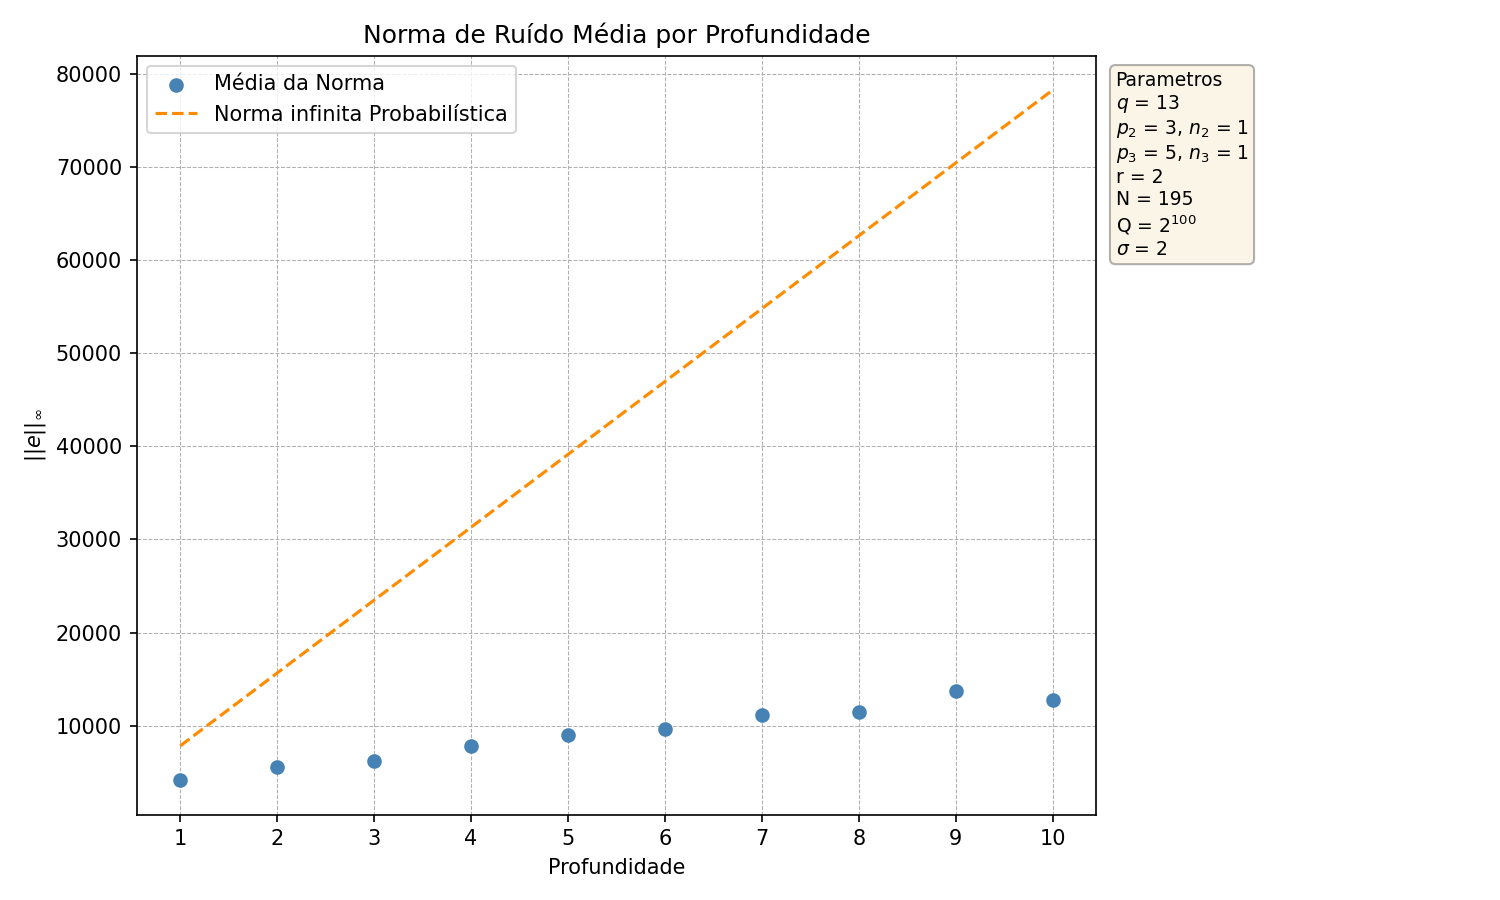
\includegraphics[width=0.8\textwidth]{images/norm.png}
    \caption{Crescimento do ruído pela quantidade de produtos externos.}
    \label{fig:norm}
\end{figure}
